% This is "sig-alternate.tex" V2.0 May 2012
% 
\documentclass{sig-alternate}

\usepackage{graphicx}
\usepackage{hyperref}
\usepackage{listings}
\lstset{basicstyle=\ttfamily,breaklines=true}

\begin{document}

\title{ScalaSCA: A Static Bug Finder for Scala\titlenote{Submitted in partial fulfilment of the requirements for CS-498 - Project in Computer Science II, at �cole Polytechnique F�d�rale de Lausanne}}


\numberofauthors{3} 
\author{
\alignauthor
Jean Andr� Gauthier\\
       \affaddr{M.S.c. Computer Science, EPFL}\\~\\
       \email{jean.gauthier@epfl.ch}
% 2nd. author
\alignauthor
Viktor Kuncak\titlenote{Professor in charge of the project}\\
       \affaddr{EPFL - Lab for Automated Reasoning and Analysis (LARA)}\\
       \email{viktor.kuncak@epfl.ch}
% 3rd. author
\alignauthor
Iulian Dragos\titlenote{Supervisor of the project}\\
       \affaddr{Typesafe Lausanne}\\~\\~\\
       \email{iulian.dragos@typesafe.com}\\
}

\makeatletter
\def\@copyrightspace{\relax}
\makeatother

\maketitle
\begin{abstract}
The aim of static code analyses is to detect programming or logic errors before execution, in order to avoid time-consuming code inspection, and most importantly to prevent errors that occur only on a small number of execution paths and might not be discovered during debugging. Unfortunately, a wide range of those static analyses are computation-intensive, and cannot be included by default as a compiler phase without disrupting the programmer's workflow. In this paper we present \textit{ScalaSCA}, a both fast and extensible static code analysis engine that is implemented as a plugin for the Scala compiler. We discuss some of the bug finding strategies we have implemented and lastly, we measure their performance overhead compared to a standard execution of the Scala compiler.
\end{abstract}

% A category with the (minimum) three required fields
\category{F.3.2.5}{Logics and Meanings of Programs}{Semantics of Programming Languages}[program analysis]

\terms{Verification, Measurement}

\keywords{Static Analysis, Scala, Testing}

\section{Introduction}

In an ideal world, software engineers would be fully reliable and commit no errors at all while developing their software. Since this is obviously not the case, the best they can do is to try to limit the occurrence of such bugs and to standardise the processes of error reporting. This is critical for minimising the amount of time a given bug is left unpatched, and leads to a greater satisfaction of the private or corporate end-users.

As shown in Figure \ref{bugs-table}, the later the stage at which a coding (or design) error is detected, the higher the cost associated to its resolution. Hence, it would make make sense to introduce additional checks at the first machine-level stage, i.e. construction, in order to prevent at least some of the bugs that would usually be detected at later stages of software development. As an example, "one in a million" errors that only occur on very few execution paths.

There exist several ways to tackle those issues, each of which has its specific advantages and disadvantages:
\begin{itemize}
\item Manual code review: as developers are notoriously poor at discovering their own bugs, this often implies that two or several developers mutually review their code. But such reviews are often time-consuming (and thus costly), and due to the sheer sizes and complexities of the codebases, very few errors are actually discovered which leads to a poor cost to bug discovery ratio.
\item Dynamic code analysis: as a first step towards code analysis automation, these analysers\footnote{Cf. \cite{nn07} for the presentation of Valgrind, a collection of dynamic code analysis tools for the C language.} rely on test cases or interactive input during the execution of the target program. Typically, debuggers fall into this category of analysers. While these tools are particularly useful when resolving memory management issues or any dynamic problems involving e.g. reflection, they do not guarantee a complete code coverage for their analysis.
\item Static code analysis: on the other side of the spectrum, static code analysers do not execute the target code at all. This has the consequence that these tools tend to be less suited to the task of solving concurrency or memory issues.\footnote{It should however be noted that this field is an active area of research and there indeed exist techniques that allow a static analysis for potential concurrency issues, as presented in \cite{ww05} for example} Static code analysers are nevertheless an invaluable tool, inasmuch that they usually have a complete code coverage.
\end{itemize}

Ideally, a static code analyser would produce a correctness proof about the code in question. Unfortunately, this is currently infeasible due to the complexity of this task. A more promising approach are correctness proofs about a reduced number of properties, usually specified as assertions. The task of the static analyser is then reduced to proving that the assertion's predicate holds on all execution paths, where relatively good results can be obtained. \footnote{The Leon verification system for Scala is an example of such a tool. \cite{vk13}} A last category of analysers does not try to provide proofs at all but rather flags probable bugs, which is the approach chosen for \textit{ScalaSCA}.

\begin{figure}
\centering
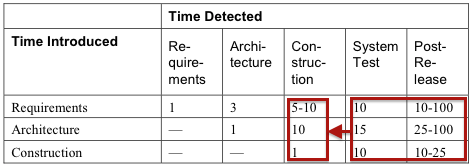
\includegraphics[width=\columnwidth ]{bugs-table.png}
\caption{Cost reduction through bug detection at construction time \cite{smc04}}
\label{bugs-table}
\end{figure}

However, it is important to remember that in practice, code analysis tools are measured against two metrics only, when being integrated in software development cycles:
\begin{itemize}
\item False positives: If the analyser produces too many unnecessary warnings, developers tend to start ignoring them, and this effectively nullifies the purpose of the tool.
\item Execution time: If on the other hand the analyser takes too long to run, it is likely to be taken out of the iterative software development cycle and run too rarely to be helpful in preventing common coding errors.
\end{itemize}
Thus, a static analyser has to strike a balance between performance and accuracy in order to be used in the most effective manner, i.e. during each codebase compilation. This explains why we deliberately oriented the development of \textit{ScalaSCA}'s towards unsound code analyses, in an attempt to improve performance at the expense of making the tool slightly less accurate.

\section{ScalaSCA internals}

\textit{ScalaSCA} has been implemented in order to provide a standardised framework for bug finding strategies. This allows an easier sharing of those strategies across the community, and simplifies the task of programming personalised strategies, if needed.

So-called "rules" are the core component of  \textit{ScalaSCA}, as they represent code snippets that perform a specific code analysis. In order to unify the referencing of each one of the rules and allow an easier lookup in bug trackers, a unique identifier has been attributed to each rule, much in the style of \textit{Findbugs} \cite{dhwp04}. \textit{ScalaSCA} differentiates between two types of rules, i.e. rules that can be applied directly on abstract syntax trees (inheriting from the \textbf{ASTRule} class) and general rules (which inherit from \textbf{StandardRule} class).


Not all categories of rules can be expressed easily

\subsection{Personalised rules}

\textit{ScalaSCA} allows the inclusion of independently developed rules by passing the \lstinline{-P:scalasca:c:<config-file-path>} to \textit{scalac} when using \textit{ScalaSCA}.

\section{Example Rules}

Broadly speaking, we have implemented three types of rules:
\begin{itemize}
\item Syntactic Rules: these rules work exclusively on ASTs, and do not rely on any intermediate representation.  GEN\_BLOCK\_CONST\_PROP
\item Control-flow rules:
\item Data-flow rules:
\item Code metrics:
\end{itemize}
\subsection{AST Rules}

\subsection{The Rule Engine}

\section{Implementation}

\textit{ScalaSCA} has been made available free of charge at \url{https://github.com/jean-andre-gauthier/scalasca}, under the 3-clause BSD license. The current implementation is entirely written in Scala, and does not make use of any additional libraries other than the standard Scala library and the Scala compiler library.

As \textit{ScalaSCA} has been developed using the \textit{sbt} interactive build tool, it provides out-of-the-box integration with any existing \textit{sbt} project by simple addition of the following line to any \textit{sbt} project configuration file:
\begin{lstlisting}
addCompilerPlugin("lara.epfl"%%"scalasca"%"0.1")
\end{lstlisting}
This will automatically run the \lstinline{DefaultRule} from \textit{ScalaSCA}. In order to change this behaviour, one or several personalised rules can be set up, compiled to \textit{jar} files and their paths stored line by line in a configuration file. This rules can then be accessed by \textit{ScalaSCA} by specifying the \lstinline{-P:scalasca:c:<config-file-path>} option.

As an example, in an \textit{sbt} configuration file, this option would be specified as follows:
\begin{lstlisting}
scalacOptions <<= (scalacOptions, scalaSource in Compile) { (options, base) =>
    options :+ ("-P:scalasca:c:" + configFilePath)
}
\end{lstlisting} 

For additional details, a sample \textit{ScalaSCA} plugin project has been made available online, at \url{https://github.com/jean-andre-gauthier/scalasca-plugin}.

\section{Performance}

\section{Related work}

Research in static code analysis has been conduced for most programming languages, one of the earliest examples being the \textit{lint} checker for the \textit{C} programming language \cite{sj78}. \textit{lint} inspired many code analysis tools, such as \textit{splint} \cite{de02} for example, whose philosophy is to avoid false positives at all costs. Among others, \textit{Goanna} for \textit{C++} \cite{rh08} takes an interesting approach as it is based on a model checker (\textit{NuSMV}) but still manages to produce relatively good performance. Much work has also been dedicated to the \textit{Java} programming language, and various tools have been developed, such as \textit{FindBugs} \cite{dwhp04} that focuses on simplicity over complexity, or \textit{soot} \cite{vr99} which is a framework that provides intermediate representations of java bytecode. \textit{ScalaSCA} is not the first foray into static analysis on Scala code, and some more complex tools that stay accurate even in the presence of first-class functions are available, e.g. \textit{Insane} \cite{vk14}. Dynamic programming languages have features which tend to complicate static analyses, as they generally expose less information to the analyser. Previous research has been investigating static analysis for languages such as PHP \cite{vk10} or Javascript \cite{shj09}.

\bibliographystyle{abbrv}
\bibliography{paper}

\end{document}
